\documentclass[11pt, a4paper]{article}
\usepackage{pdfpages}
\usepackage{parallel}
\usepackage[T2A]{fontenc}
\usepackage{ucs}
\usepackage[utf8x]{inputenc}
\usepackage[polish,english,russian]{babel}
\usepackage{hyperref}
\usepackage{rotating}
\usepackage[inner=2cm,top=1.8cm,outer=2cm,bottom=2.3cm,nohead]{geometry}
\usepackage{listings}
\usepackage{graphicx}
\usepackage{wrapfig}
\usepackage{longtable}
\usepackage{indentfirst}
\usepackage{array}
\usepackage{tikzsymbols}
\usepackage{soul}
\usepackage[ruled,vlined]{algorithm2e}
%\counterwithout{figure}{section} 

\usepackage{url}
\makeatletter
\g@addto@macro{\UrlBreaks}{\UrlOrds}
\makeatother

\newcolumntype{P}[1]{>{\raggedright\arraybackslash}p{#1}}
\frenchspacing
\usepackage{fixltx2e} %text sub- and superscripts
\usepackage{icomma} % коскі ў матэматычным рэжыме
\PreloadUnicodePage{4}

\newcommand{\longpage}{\enlargethispage{\baselineskip}}
\newcommand{\shortpage}{\enlargethispage{-\baselineskip}}

\def\switchlang#1{\expandafter\csname switchlang#1\endcsname}
\def\switchlangbe{
\let\saverefname=\refname%
\def\refname{Літаратура}%
\def\figurename{Іл.}%
}
\def\switchlangen{
\let\saverefname=\refname%
\def\refname{References}%
\def\figurename{Fig.}%
}
\def\switchlangru{
\let\saverefname=\refname%
\let\savefigurename=\figurename%
\def\refname{Литература}%
\def\figurename{Рис.}%
}

\hyphenation{admi-ni-stra-tive}
\hyphenation{ex-pe-ri-ence}
\hyphenation{fle-xi-bi-li-ty}
\hyphenation{Py-thon}
\hyphenation{ma-the-ma-ti-cal}
\hyphenation{re-ported}
\hyphenation{imp-le-menta-tions}
\hyphenation{pro-vides}
\hyphenation{en-gi-neering}
\hyphenation{com-pa-ti-bi-li-ty}
\hyphenation{im-pos-sible}
\hyphenation{desk-top}
\hyphenation{elec-tro-nic}
\hyphenation{com-pa-ny}
\hyphenation{de-ve-lop-ment}
\hyphenation{de-ve-loping}
\hyphenation{de-ve-lop}
\hyphenation{da-ta-ba-se}
\hyphenation{plat-forms}
\hyphenation{or-ga-ni-za-tion}
\hyphenation{pro-gramming}
\hyphenation{in-stru-ments}
\hyphenation{Li-nux}
\hyphenation{sour-ce}
\hyphenation{en-vi-ron-ment}
\hyphenation{Te-le-pathy}
\hyphenation{Li-nux-ov-ka}
\hyphenation{Open-BSD}
\hyphenation{Free-BSD}
\hyphenation{men-ti-on-ed}
\hyphenation{app-li-ca-tion}

\def\progref!#1!{\texttt{#1}}
\renewcommand{\arraystretch}{2} %Іначай формулы ў матрыцы зліпаюцца з лініямі
\usepackage{array}

\def\interview #1 (#2), #3, #4, #5\par{

\section[#1, #3, #4]{#1 -- #3, #4}
\def\qname{LVEE}
\def\aname{#1}
\def\q ##1\par{{\noindent \bf \qname: ##1 }\par}
\def\a{{\noindent \bf \aname: } \def\qname{L}\def\aname{#2}}
}

\def\interview* #1 (#2), #3, #4, #5\par{

\section*{#1\\{\small\rm #3, #4. #5}}
\ifx\ParallelWhichBox\undefined%
    \addcontentsline{toc}{section}{#1, #3, #4}%
\else%
\ifnum\ParallelWhichBox=0%
    \addcontentsline{toc}{section}{#1, #3, #4}%
\fi\fi%

\def\qname{LVEE}
\def\aname{#1}
\def\q ##1\par{{\noindent \bf \qname: ##1 }\par}
\def\a{{\noindent \bf \aname: } \def\qname{L}\def\aname{#2}}
}

\newcommand{\interviewfooter}[1]{
\vskip 1em
\noindent \textit{#1}
}

\switchlang{ru}
\begin{document}

\title{1986 "--- Commodore C300 mouse}
\date{}
\maketitle
\selectlanguage{russian}
Мышь Commodore C300 mouse, подписанная на коробке как Joystick Mouse "--- это одна из реинкарнаций Kempston Mouse, выпущенной в 1986 году для компьютеров ZX Spectrum \cite{SinclairUser}, адаптированная для компьютеров Commodore \cite{c64wiki}. Внешне мышь является достаточно типичной, с двумя кнопками на верхней стороне и шаром снизу (рис. \ref{fig:C300Pic}).

\begin{figure}[h]
    \centering
    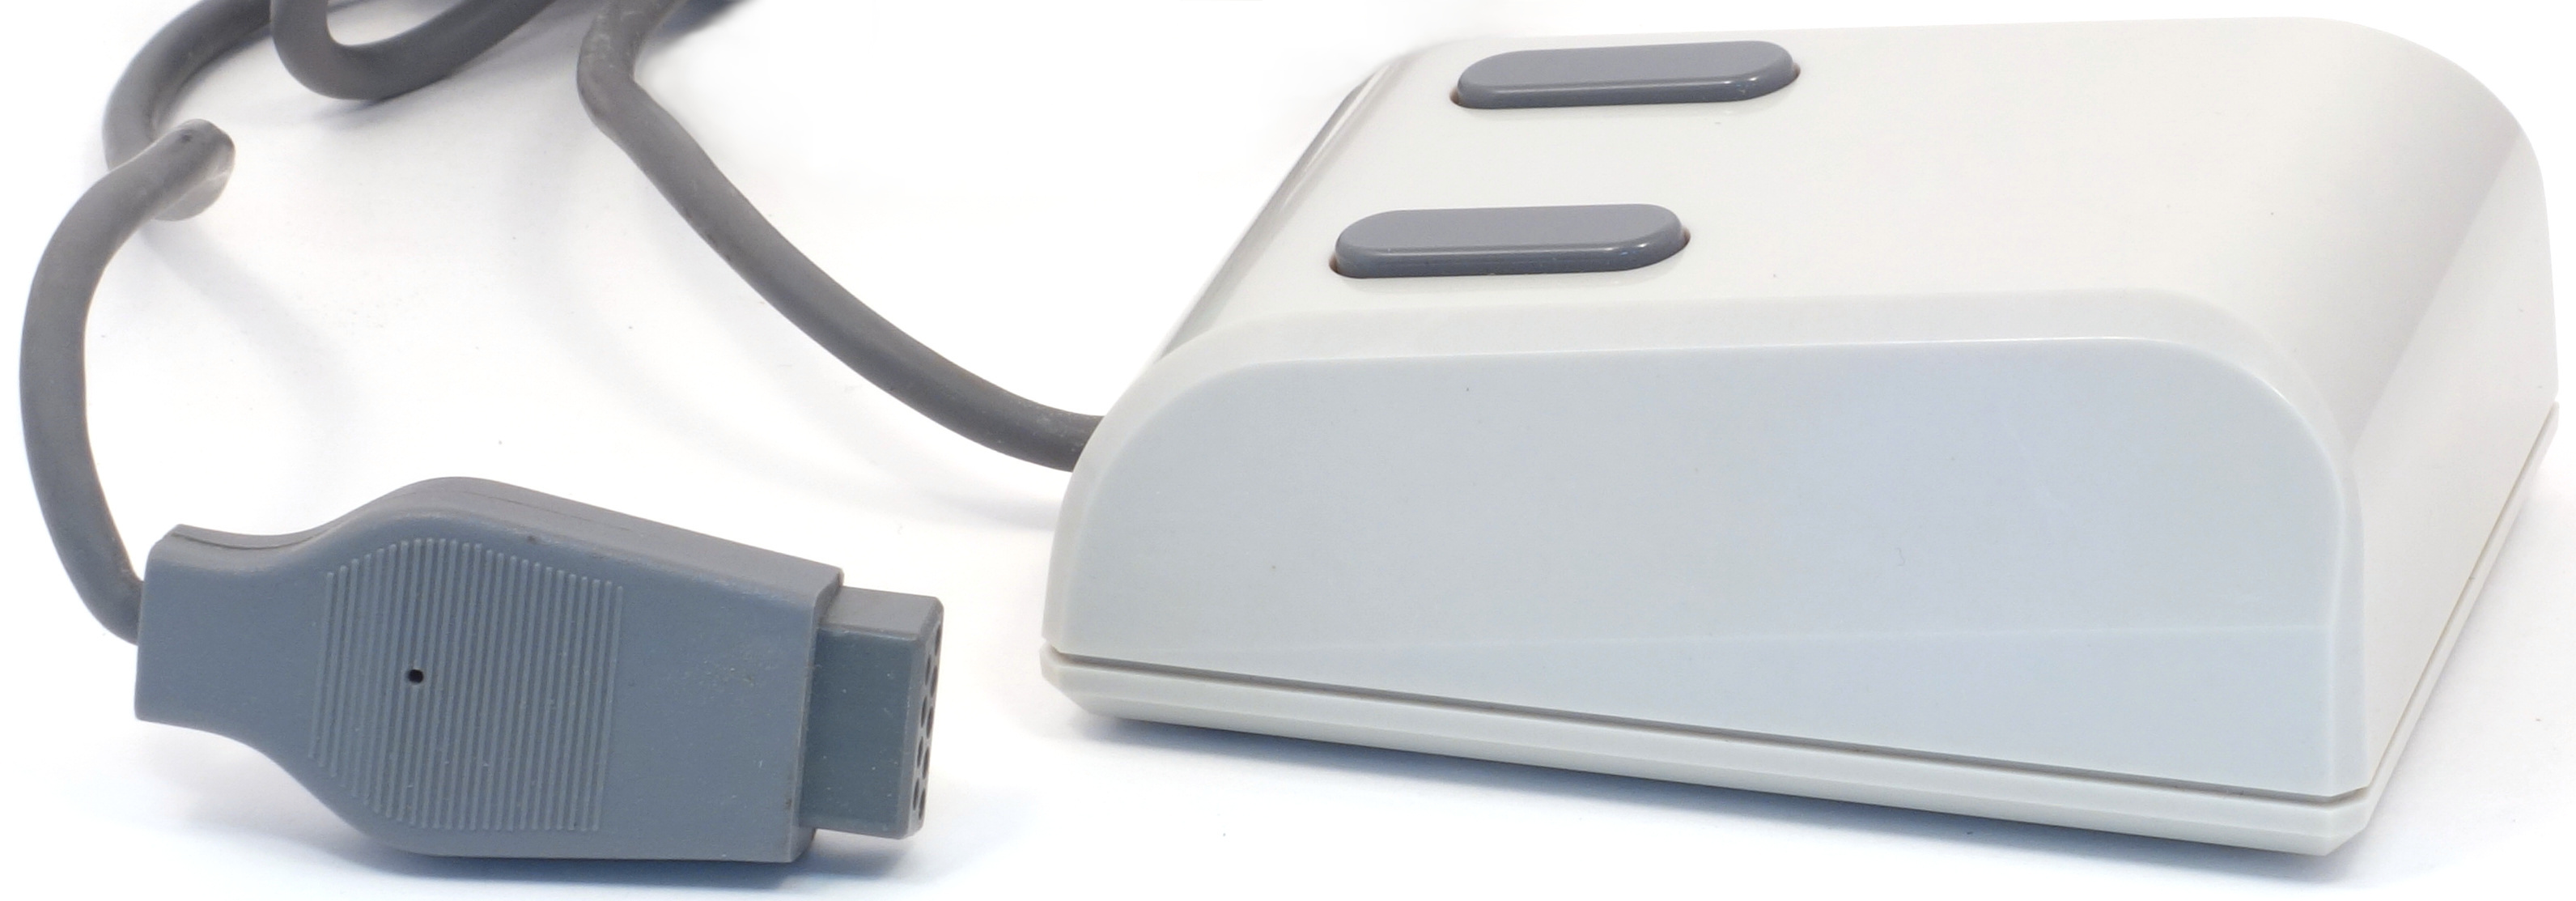
\includegraphics[scale=0.7]{1986_commodore_c300_mouse/cmnirm_30.jpg}
    \caption{Commodore C300 Mouse}
    \label{fig:C300Pic}
\end{figure}

Согласно прилагаемому описанию, данная мышь работает в двух режимах работы: в режиме джойстика и пропорциональном режиме. Режим работы определяется при включении компьютера: при нажатии правой кнопки мыши мышь переходит в режим джойстика, в противном случае (по умолчанию) в пропорциональный режим. В режиме джойстика левая кнопка мыши задействована как кнопка включения джойстика, а правая кнопка эквивалентна движению джойстика вверх. Режим джойстика позволяет использовать мышь с любым программным обеспечением, совместимым с джойстиком, а также играет роль <<резерва>> на случай, когда используемое программное обеспечение не поддерживает пропорциональный режим.


\begin{figure}[h]
    \centering
    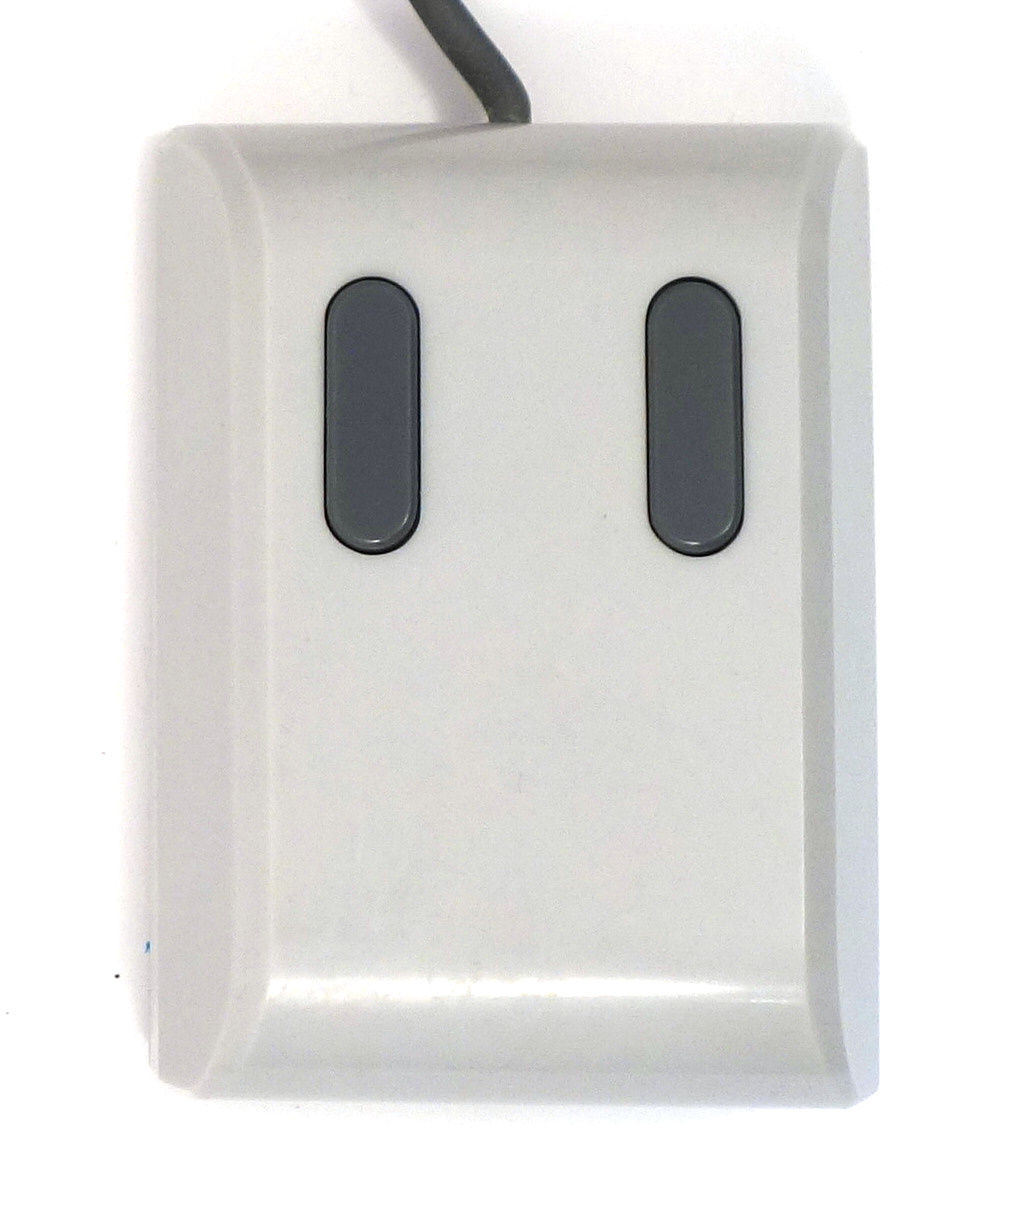
\includegraphics[scale=0.7]{1986_commodore_c300_mouse/3verh_60.jpg}
    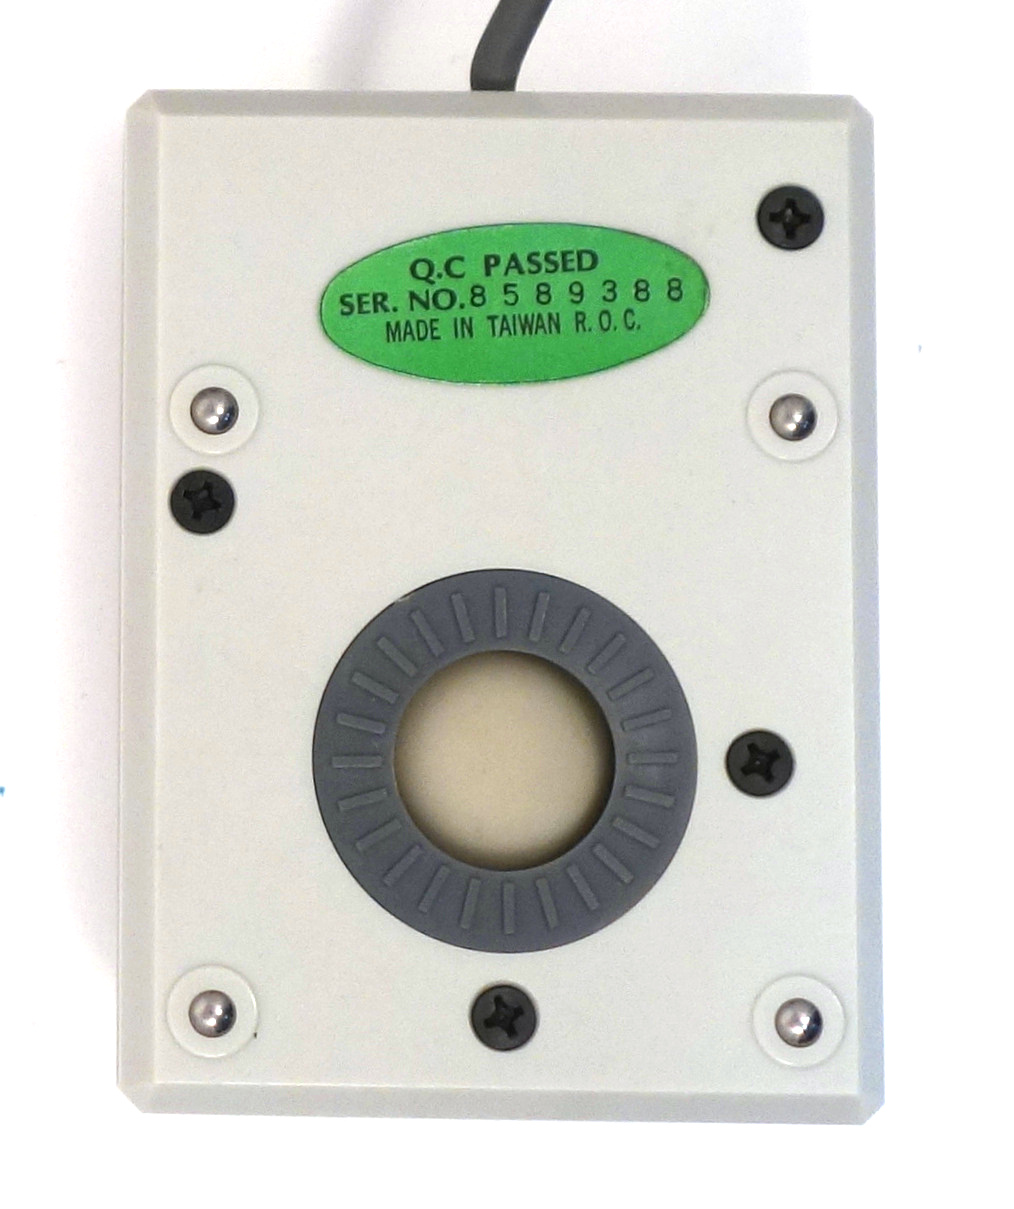
\includegraphics[scale=0.7]{1986_commodore_c300_mouse/3niz_60.jpg}
    \caption{Commodore C300 Mouse, вид сверху и снизу}
    \label{fig:C300TopAndBottom}
\end{figure}

Как иможно заметить на рис. \ref{fig:C300TopAndBottom}, плавное скольжение мыши по рабочей поверхности обеспечивается не тканевыми накладками с низким коэффициентом сопротивления или пластиковым <<ножками>>, а четырьмя металлическими шариками малого диаметра, расположенными в дополнительных отверстиях нижней стенки корпуса и свободно вращающимися при движении (решение, характерное для ряда механических мышей 80-х годов, выпускавшихся до ряда изменений типовой конструкции, направленных на удешевление изделий).

\begin{figure}[h]
    \centering
    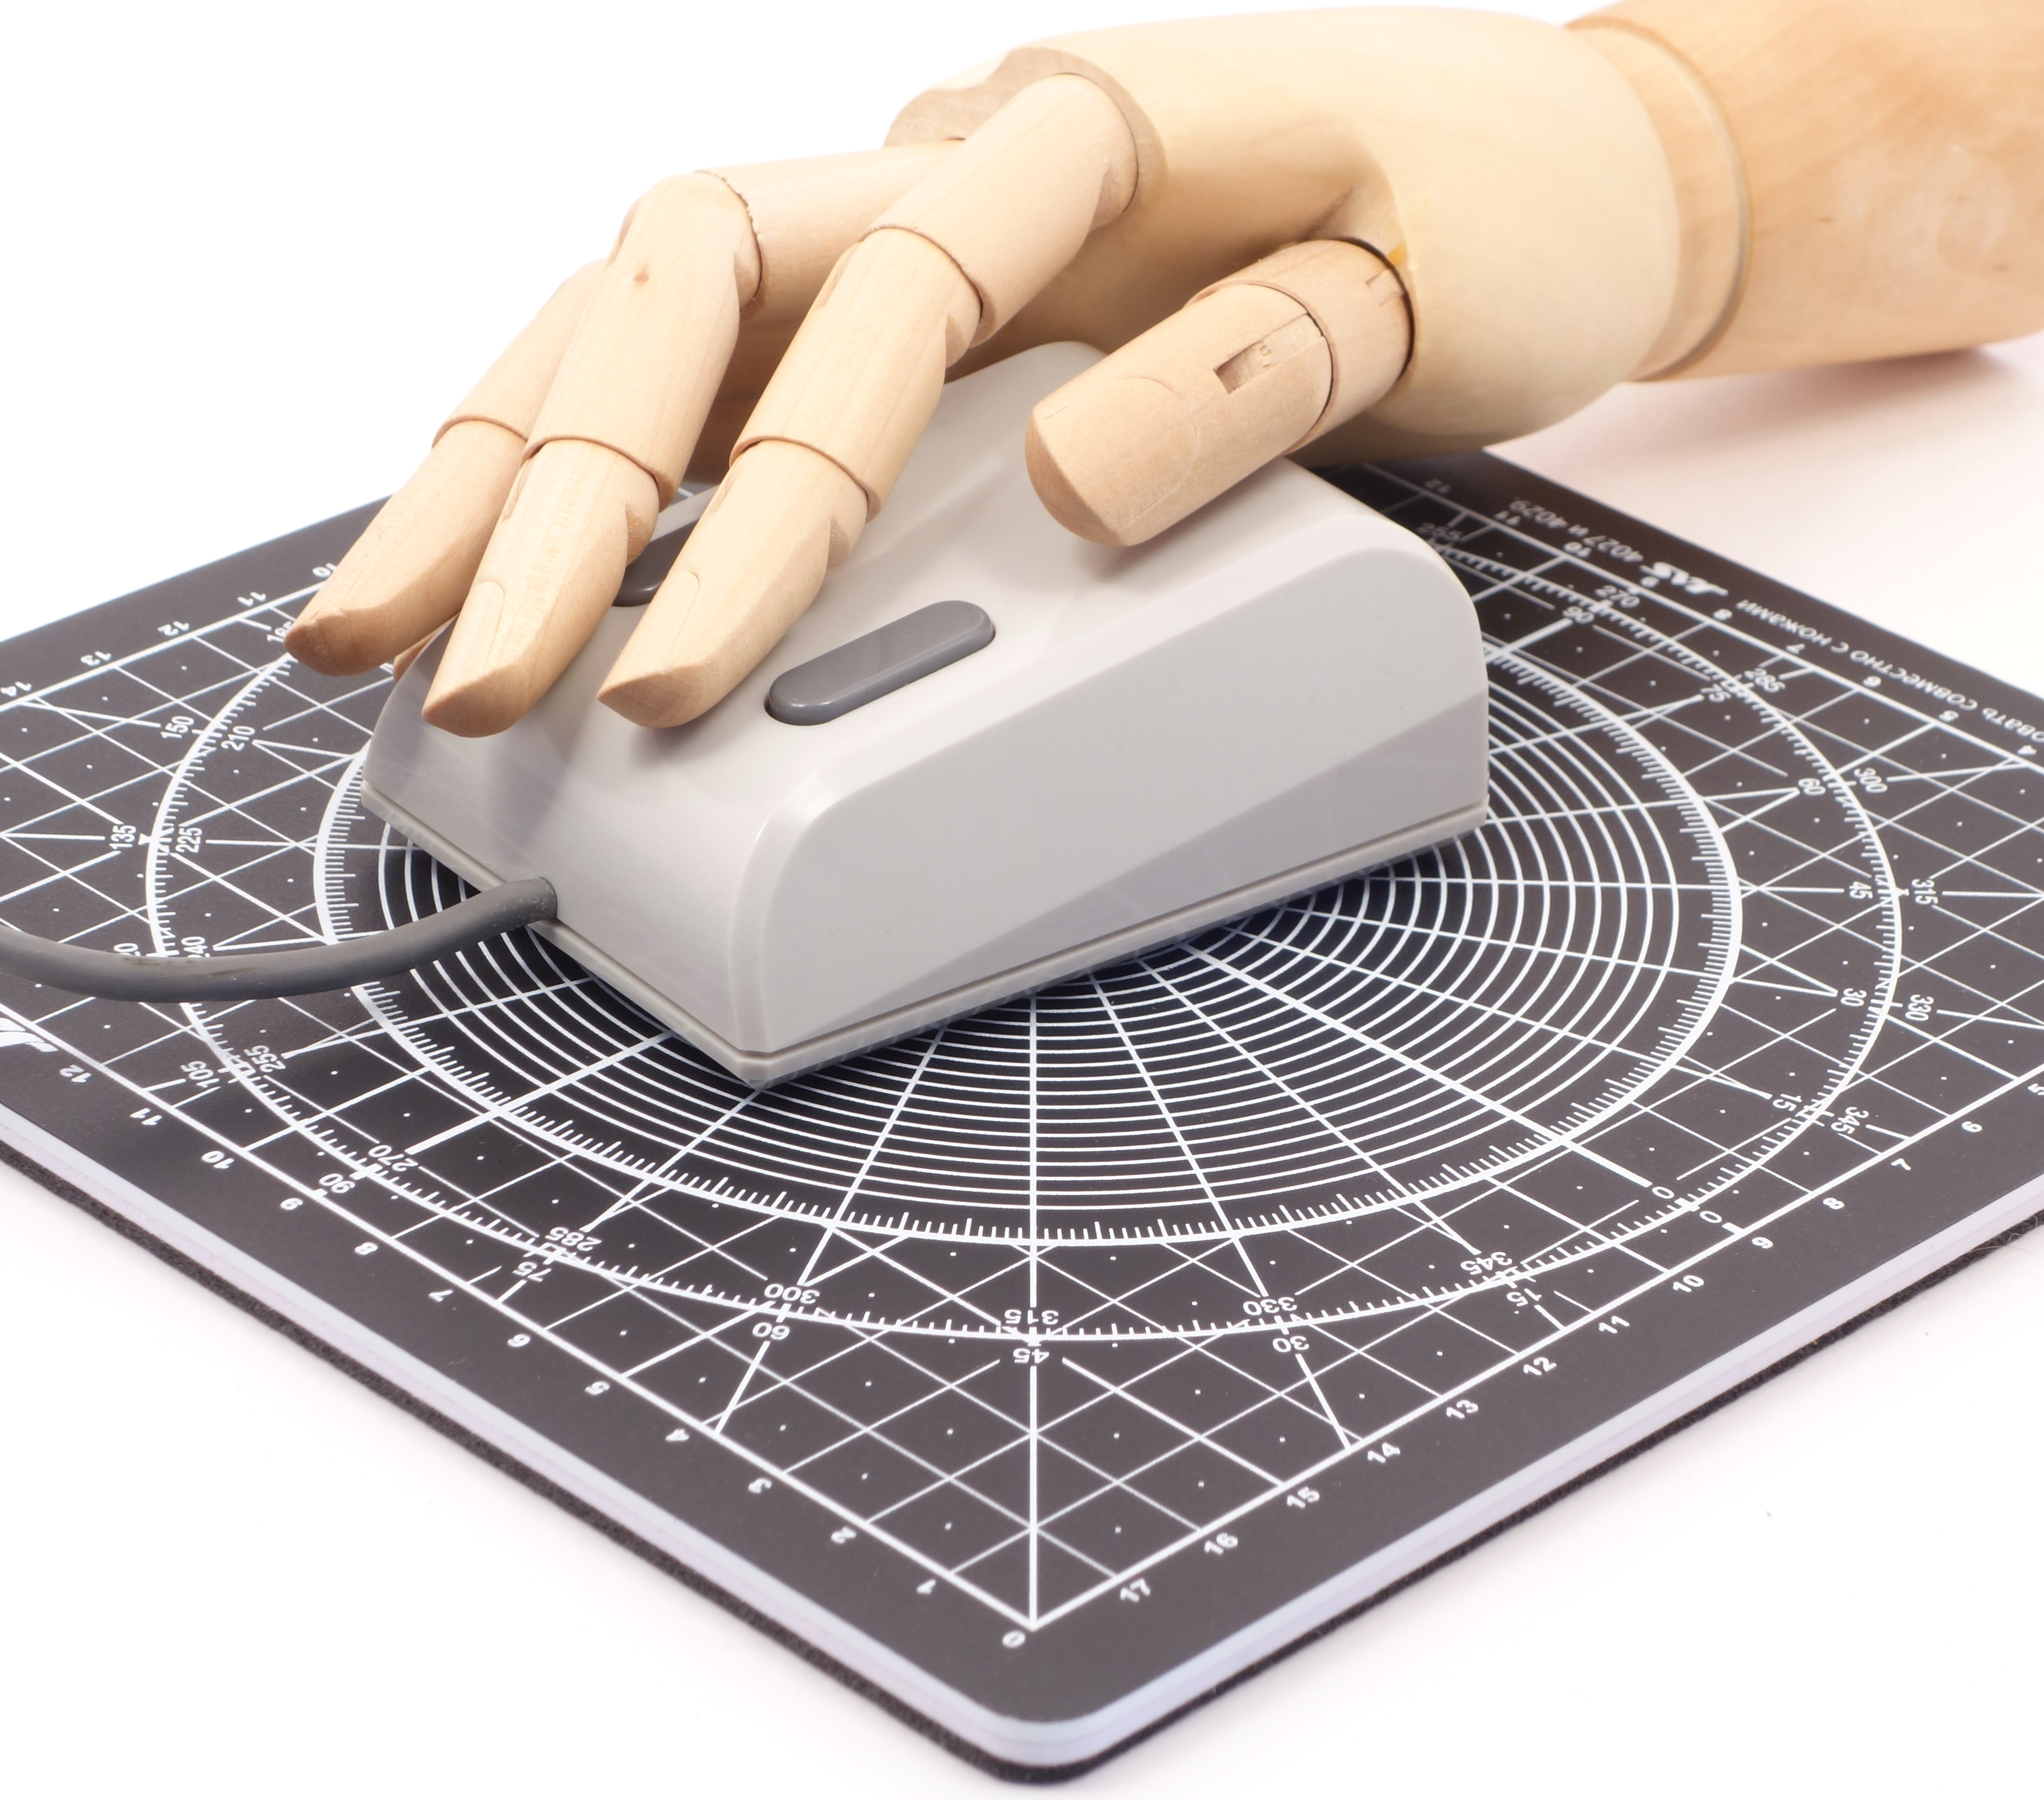
\includegraphics[scale=0.3]{1986_commodore_c300_mouse/cmruka_30.jpg}
    \caption{Commodore C300 Mouse с моделью руки человека}
    \label{fig:C300Hand}
\end{figure}

\begin{figure}[h]
    \centering
    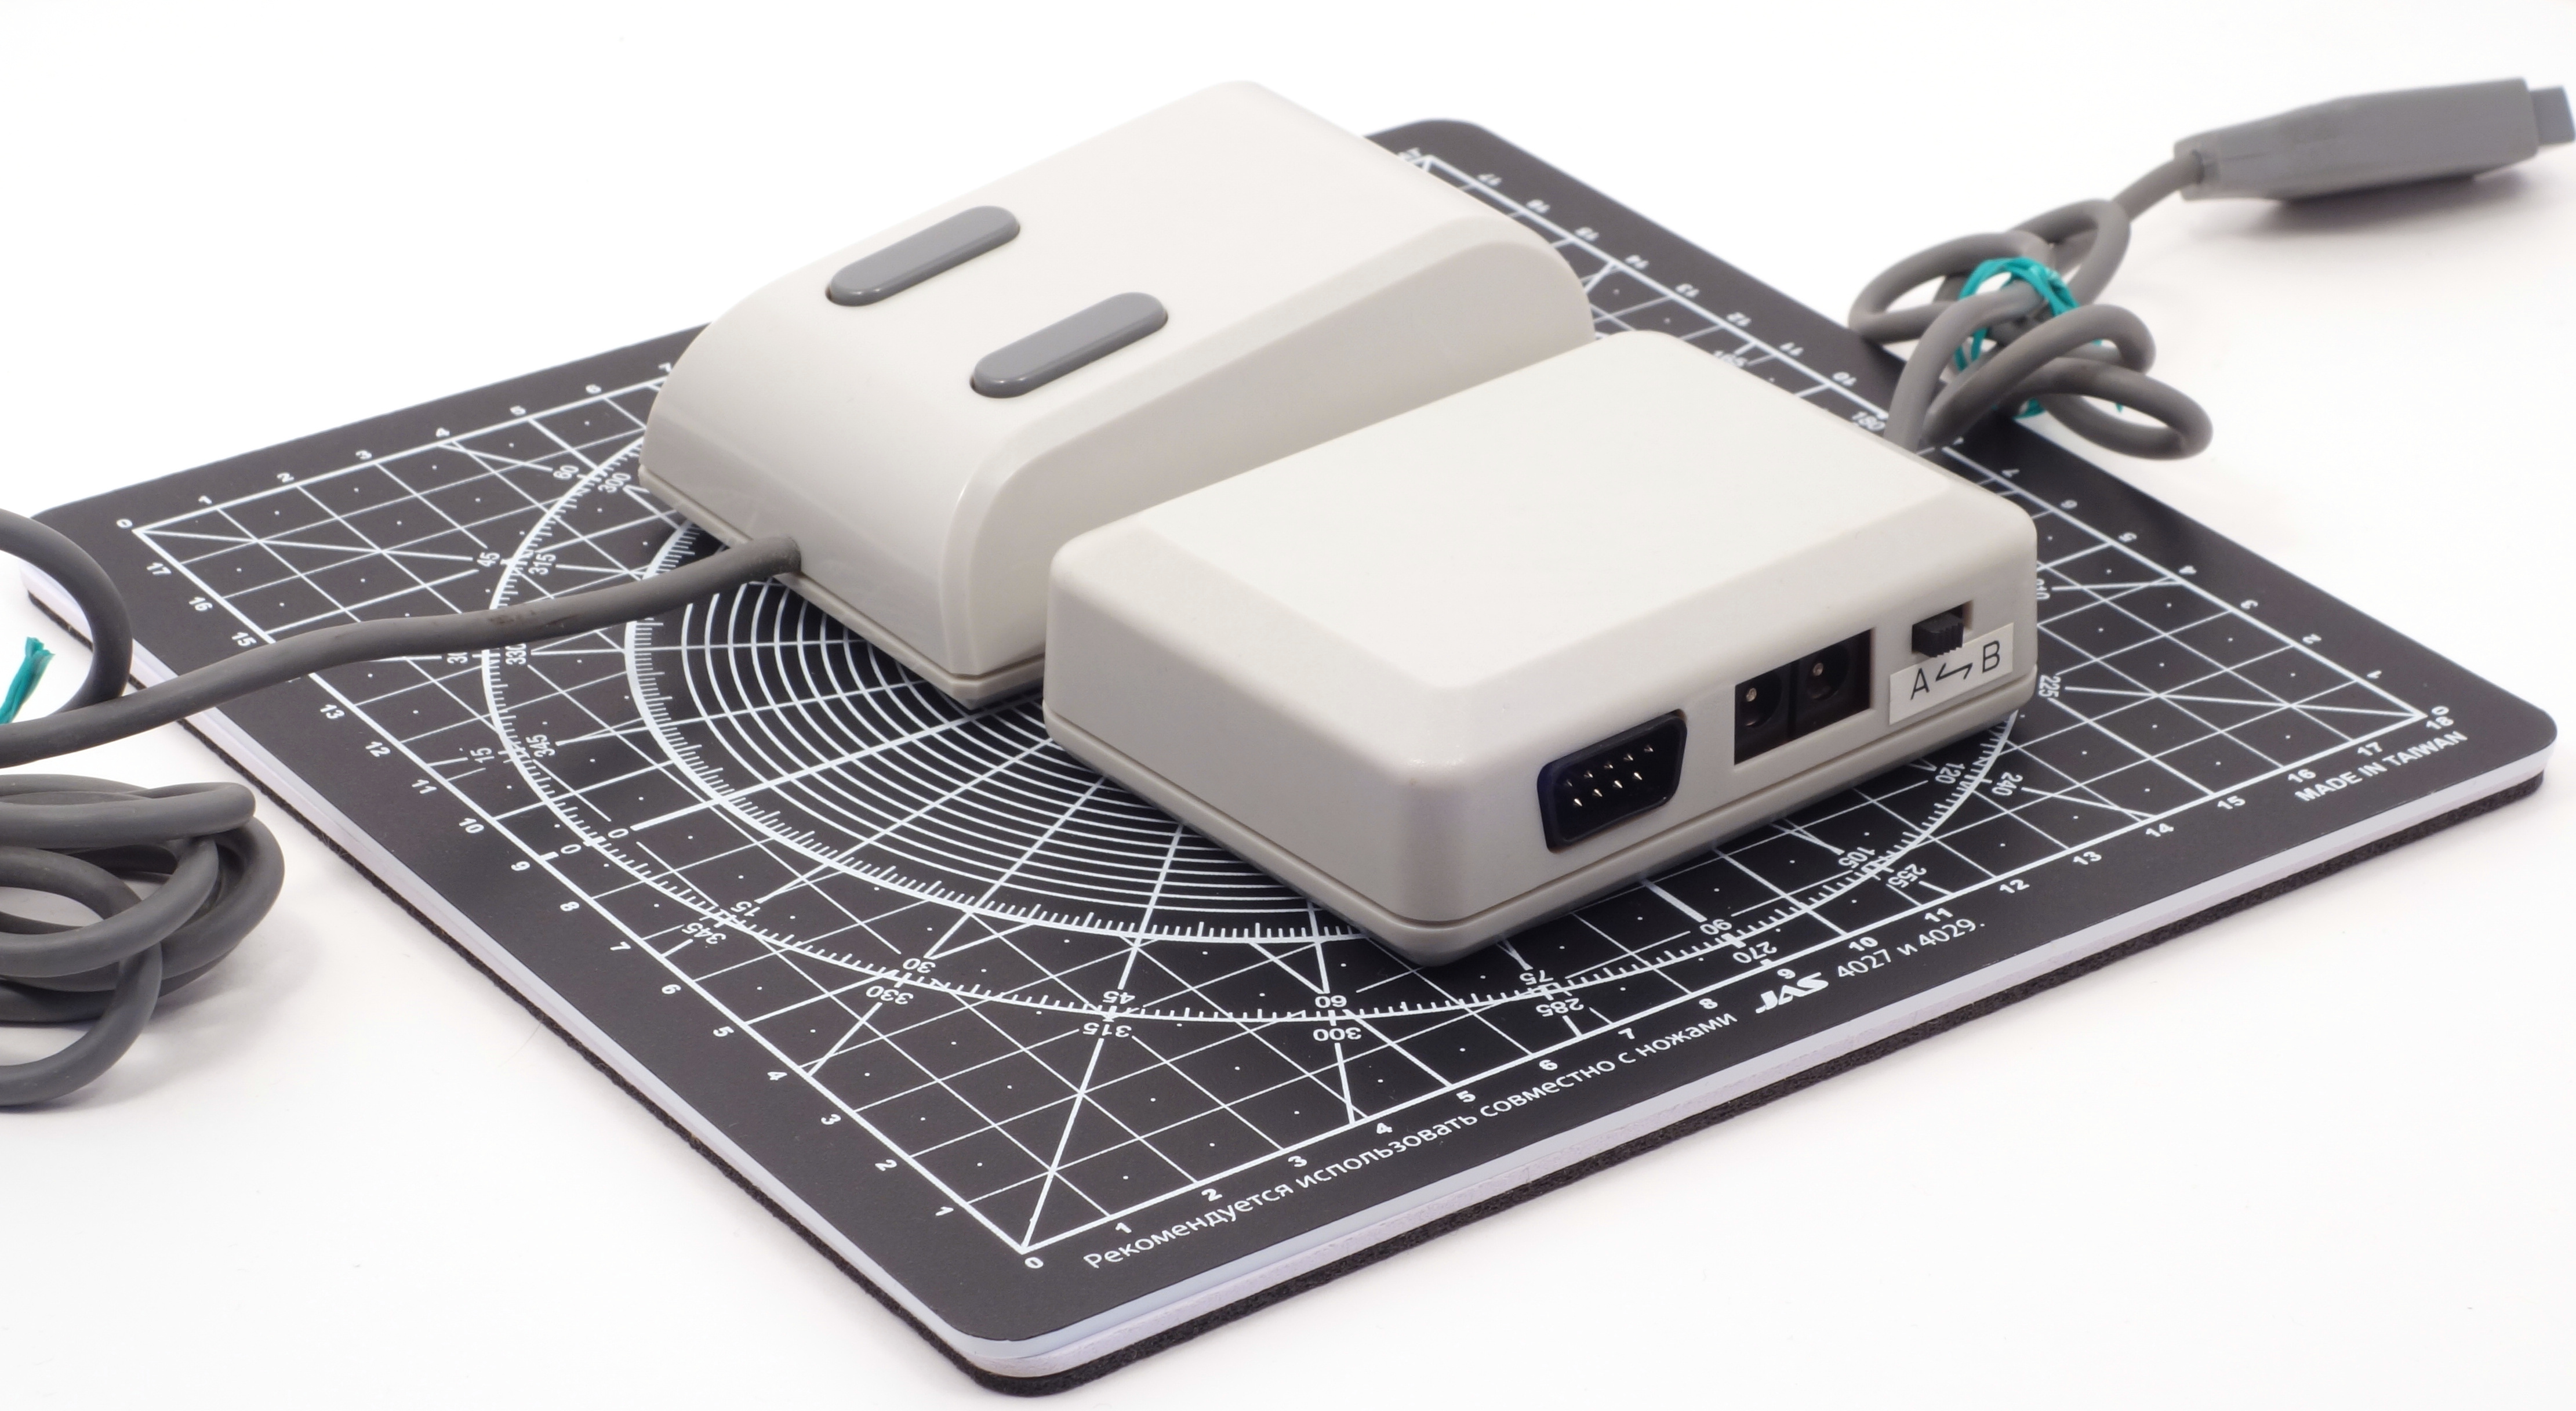
\includegraphics[scale=0.3]{1986_commodore_c300_mouse/cmblock_30.jpg}
    \caption{Адаптер Commodore, вид спереди}
    \label{fig:C300Block}
\end{figure}

\begin{figure}[h]
    \centering
    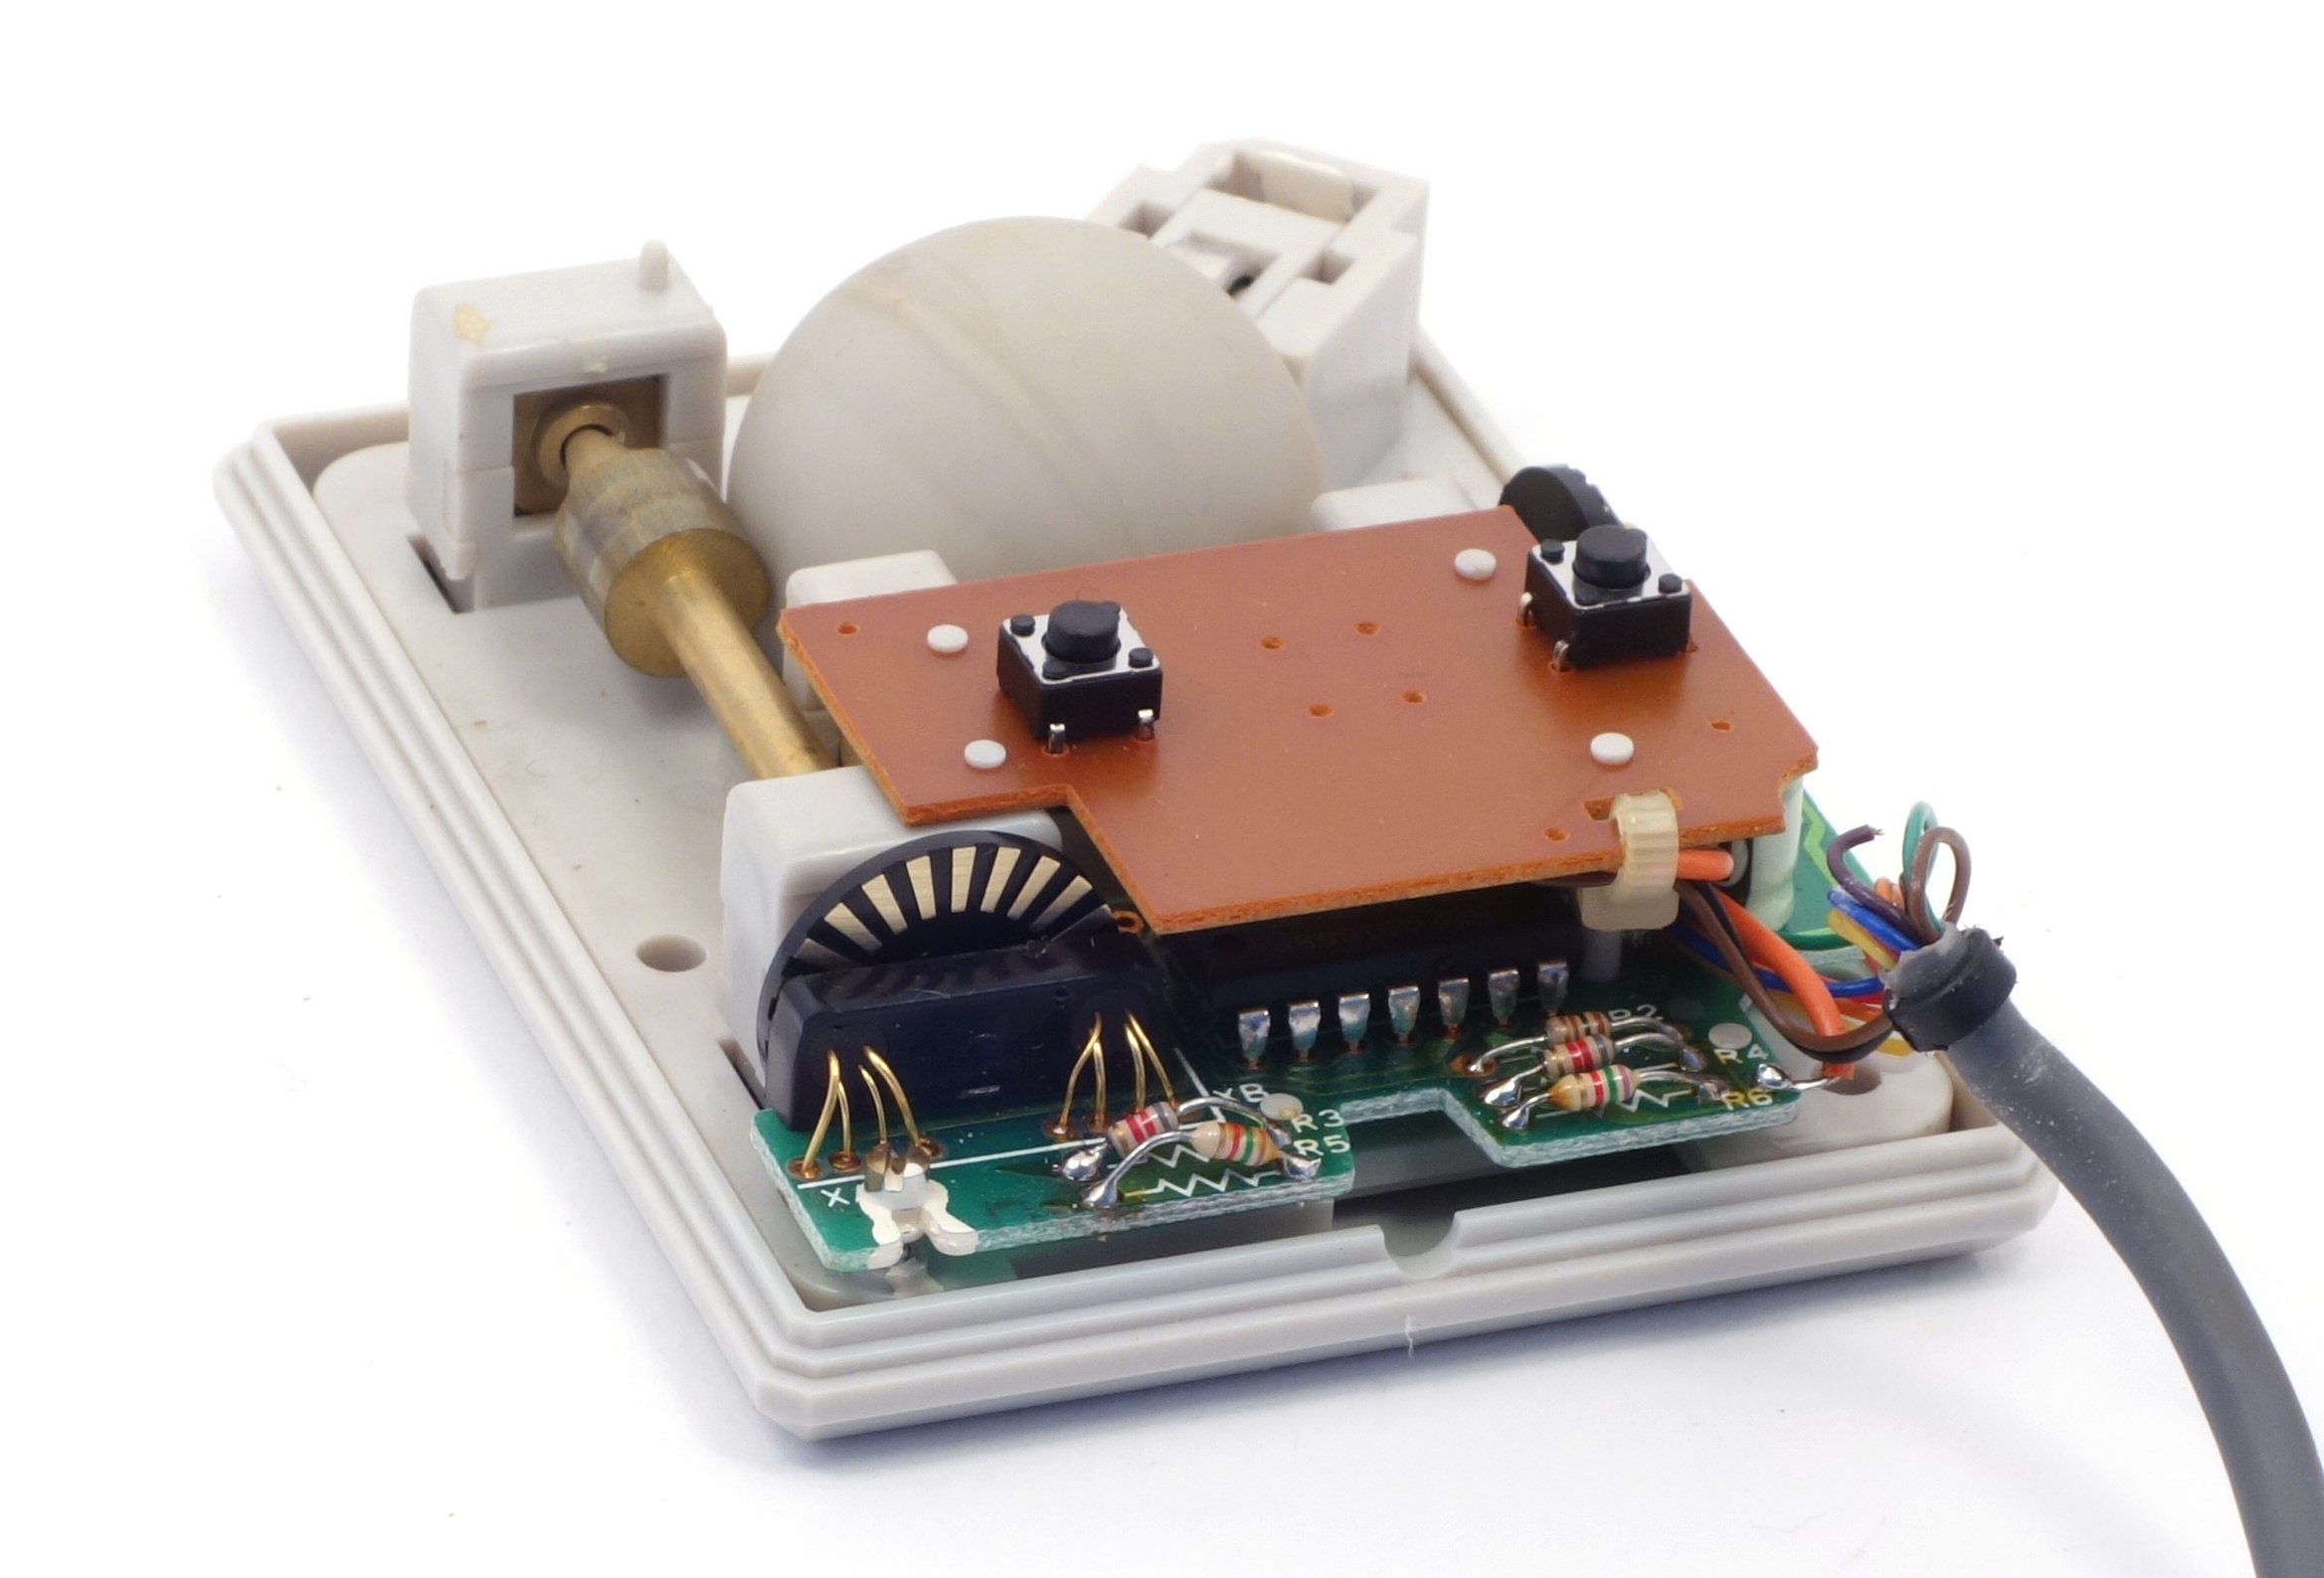
\includegraphics[scale=0.7]{1986_commodore_c300_mouse/cm4raz_30.jpg}
%    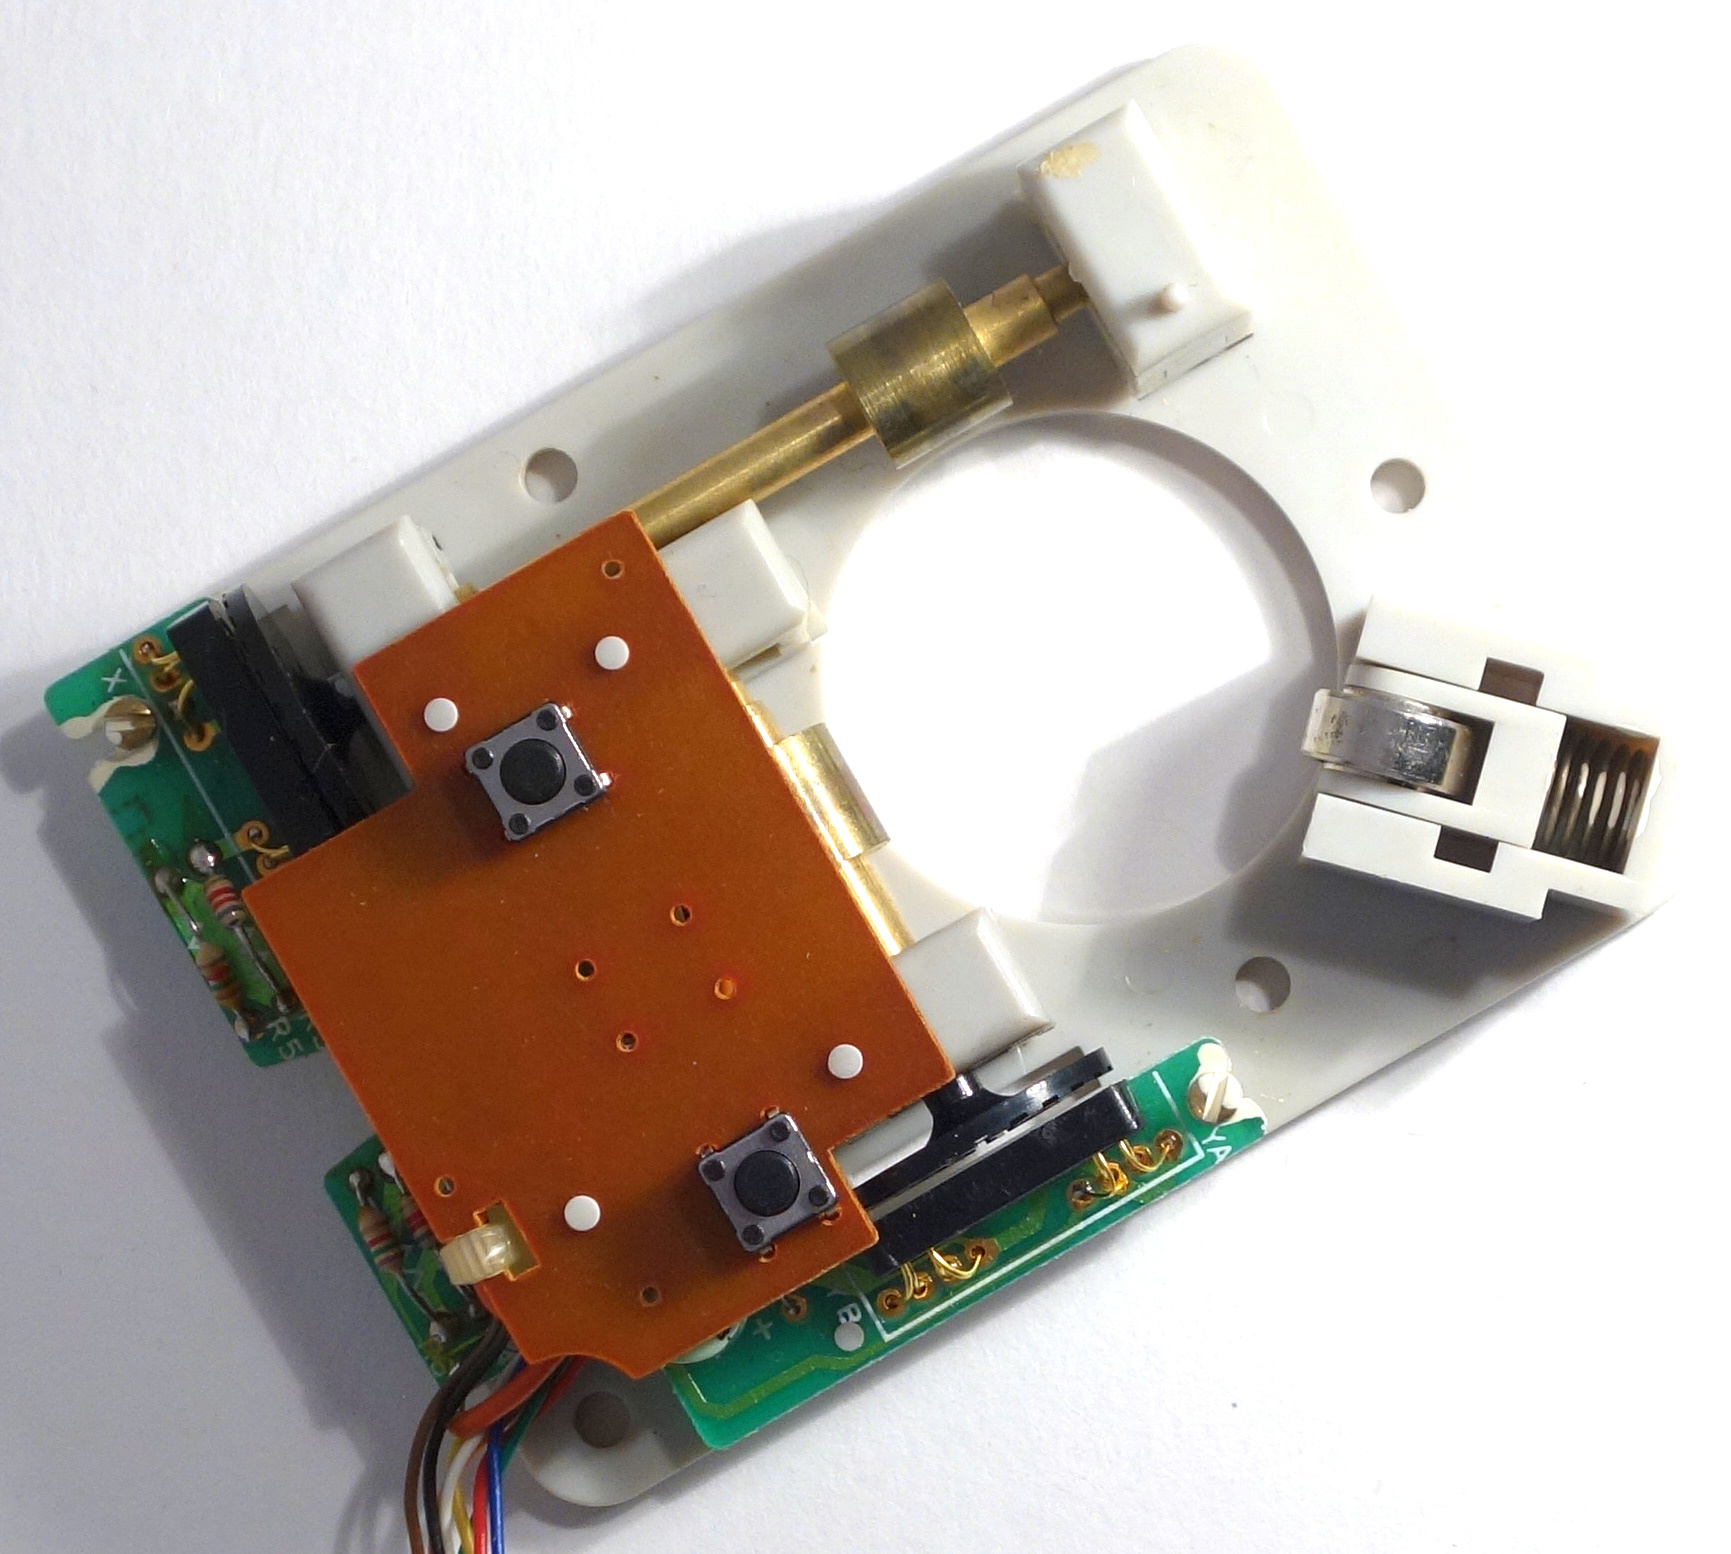
\includegraphics[scale=0.7]{1986_commodore_c300_mouse/cm41raz_30.jpg}
    \caption{Commodore C300 Mouse в разобранном виде}
    \label{fig:C300Inside}
\end{figure}

Разбор мыши показывает достаточно необычную конструкцию (рис. \ref{fig:C300Inside}): это оригинальное оптомеханическое указательное устройство, в котором нестандартно реализован оптический прерыватель. Вместо прохождения диска между источником и приёмником света, светодиод и фотодиод располагаются по одну и ту же сторону диска, а сам диск является сплошным. Вместо прорезей, в нём использованы радиальные металлические полосы, отражающие свет, в то время как черный матовый материал самого диска рассеивает его, приводя к отсутствию сигнала на фотоприёмнике. В электрическом плане подобная конструкция не отличается от других оптомеханических мышей, но визуально напоминает диск контактного энкодера (в случае которого при механическом контакте щёток с поверхностью диска происходило бы замыкание цепи в момент прохождения металлической радиальной полосы и её размыкание когда щётка оказывалась между полосами).

Безусловно, такое решение не является дешёвым в сравнении с традиционной схемой, использующей пластиковый диск с прорезями без металлизации.

\begin{thebibliography}{9}
\bibitem {c64wiki} Mouse -- C64-Wiki \url{https://www.c64-wiki.com/wiki/Mouse}
\bibitem {SinclairUser} Kempston mouse // Sinclair User, Iss. 56, November 1986. -- p. 29. \url{https://worldofspectrum.org/archive/magazines/sinclair-user/56/0/1986/11/0}
\end{thebibliography}
\end{document}
